\chapter{Introduction}
\label{chap:introduction}
In this work we experiment in formal verification of Scala code. 
We use the verification framework Stainless to verify the code of Bitcoin-S-Core, the Scala implementation of the Bitcoin protocol.
In the following we describe the main aspects of formal verification, Stainless and the project Bitcoin-S.


\section{What is formal verification}
\label{sec:formal_verification}

The longer and more complex a source code is, the more difficult it is to verify its correctness.
There are different approaches for verification of the program correctness. 

The commonly used one is testing.
A developer creates a set of some practical scenarios and assertions to test a software design and implementation. 
So, the actual results are checked to match the expected results.
Tests help to identify bugs and missing requirements.
However, not all possible inputs can be tested. 
Therefore, a long-term test coverage model is usually created to test a software design enough.
Nevertheless, this is still not easy to test a software being able to observe the side effects of a code.
\textbf{Practically, a developer runs tests, debugs appeared failures, adjusts a code and extends a test bench to verify the previously uncovered aspects. (TODO// do we need this sentence?)}\cite{sanghavi:formal_verification}

Another powerful method to check whether a program works correct is formal verification. 
This is a systematic process based on mathematical modeling. 
It is unnecessary to create a simulation tests with some possible inputs. 
With formal verification all possible input values are explored algorithmically and exhaustively.
Correctness of a program is analyzed relative to its formal specification.
Formal specification is a mathematical description of a software behavior that can be provided to the formal verification tool for proving it.\cite{sanghavi:formal_verification}

One of such tools is Stainless which we use in our work.


\section{Overview of Stainless}
\label{sec:stainless}


Stainless is developed by "Lab for Automated Reasoning and Analysis" (LARA) at EPFL's School of Computer and Communication Sciences.
Using this framework we can verify the correctness of Scala programs.
Stainless statically verifies that a program satisfies a given specification and that a program will not crash at runtime.
The framework explores all possible input values, reports inputs for which a program fails and demonstrates counterexamples which violate a given specification.\cite{Stainless:introduction}

The main functions used to write a specification are \textit{require} and \textit{ensuring}. 
With \textit{require} we define a precondition of a function, which we want to verify.
\textit{require} is called at the beginning of the function body.
A constraint for inputs to the function is passed as an argument to \textit{require} in the form of a Boolean expression.
With \textit{ensuring} we provide a postcondition which is a condition on an output of the function.
\textit{ensuring} is called after the function body.
While compiling Stainless tries to prove that the postcondition always holds, assuming the given precondition does hold.\cite{Stainless:introduction}

The following example demonstrates a simple formal specification for the function calculating factorial.
We has taken the example from the Stainless documentation \cite{Stainless:introduction} and modified it, so Stainless reports an error verifying it.

\begin{lstlisting}[language=Scala]
    def factorial(n: Int): Int = {
        require(n >= 0)
        if (n == 0) {
          1
        } else {
          n * factorial(n - 1)
        }
    } ensuring(res => res >= 0)
\end{lstlisting}

The function recursively calculates factorial of an integer number.
An input to the function is constrained with \textit{require} to a non-negative value.
A result of the calculation should be also a non-negative.
Thus, Stainless will verify whether the result of the factorial calculation is non-negative for all non-negative inputs.

Stainless can produce 3 outcomes of postcondition verification: \textit{valid}, \textit{invalid} and \textit{unknown}.
If the postcondition is \textit{valid} Stainless could prove that for any inputs constrained in the precondition, the postcondition always holds.
Reporting the postcondition as \textit{invalid} the framework could find at least one counterexample which satisfies the precondition but violates the postcondition.
If Stainless is unable to prove the postcondition or find a counterexample it reports the outcome \textit{unknown}.
In this case a timeout or an internal error has occurred.
Furthermore, Stainless verifies that the precondition cannot be violated through the calling of the function being verified with an argument out of the precondition constraint.
So, the framework reports also \textit{valid} or \textit{invalid} for the precondition. \cite{Stainless:introduction}

Let's return back to our incorrect example with factorial. While compiling Stainless disproves the postcondition and gives the number 17 as a counterexample.
The type of an argument and return value is defined as Int, which is 32 bit long.
Thus, calculating factorial of 17 causes an overflow and results to a negative value.
The program would work correct by changing a type of number to BigInt.

Stainless reports the following result of the factorial verification from our example:

\begin{figure}[H]
	\centering
		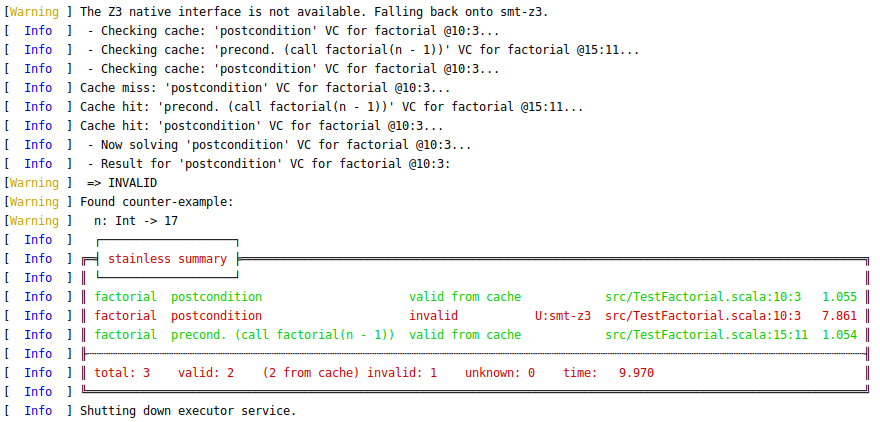
\includegraphics[scale=0.5]{images/output1.png}
	\caption{Output of Stainless verification for calculating factorial of Int number}
	\label{fig:output1}
\end{figure}


The code being verified must be written in Pure Scala, a functional subset of Scala. 
The whole specification of Pure Scala is given on the website of Stainless \cite{Stainless:pure_scala}.
Moreover, Stainless supports some imperative features translating them into Pure Scala during a preprocessing phase.
To summarise them, the following extensions to the functional Scala are available \textbf{(//TODO: may be delete it)}: 
\begin{itemize}
  \item using mutable variables in some cases
  \item using while loops
  \item gettng an old value of a variable before the execution of a function being verified
  \item using arrays that allow reassignment of its elements
\end{itemize}
The description of the supported imperative features and examples can be found on the website \cite{Stainless:imperative}. 
In addition, Stainless has its own library with annotations, reimplementaion of some core data types, collections and input-output functions and much more.
Some of them are described on the website of \cite{Stainless:library}.
More details to the library can be found in the source code of Stainless on GitHub \cite{Stainless:github} in the folder \textit{/frontends/library/stainless}.

Stainless verifies Scala programs using SMT (satisfiability modulo theories) solvers. 
The framework transforms a program code to the Pure Scala fragment supported by Inox solver.
This solver was also developed by LARA-Group and allows usage of different SMT solvers such as Z3, CVC4 and Princess, adding support of other higher-level features.
Thus, preconditions, postconditions and assertions are translated into SMT formulas, so an SMT solver can determine if all properties hold.\cite{Stainless:introduction}\cite{Stainless}


\section{Overview of Bitcoin-S}
\label{sec:bitcoin_s}

In the work some fragments of the code of Bitcoin-S has to be verified.
Bitcoin-S is an open source Scala implementation of the Bitcoin protocol. 
There are different projects belonging to Bitcoin-S.
Protocol data structures are defined in the package \textbf{bitcoin-s-core}.
This package is the main target to be verified because it specifies the base of Bitcoin protocol, and it is crucial for correct protocol functionality.
There is also the package \textbf{bitcoind-rpc} which is an RPC client implementation to communicate with \textit{bitcoind}, daemon of Bitcoin Core running on a machine.
Developers of Bitcoin-S are working on the implementation of a lightweight bitcoin client in the package \textbf{bitcoin-s-spv-node}.
The whole list of packages can be found on GitHub \cite{BitcoinSProject}.

Bitcoin-S is a large project implementing many functionalities.
In this work one of them is going to be examined and worked on, namely the property of the Bitcoin that a non-coinbase transaction can not generate new coins.
Thus, the code of Bitcoin-S should be analyzed, and fragments implementing this feature should be identified.
Afterwards, the fragments should be rewritten, so that Stainless can accept it.
After that a formal specification for functions should be defined and annotated according Stainless libraries, so that Stainless can verify correctness of the code.


